\graphicspath{{figures/appendix/}}
\chapter{Error in estimation of \gls{aoa} using \gls{adc} and multiplication method}\label{appendix:aoaestimationerr}
\begin{figure} [h]
\centering
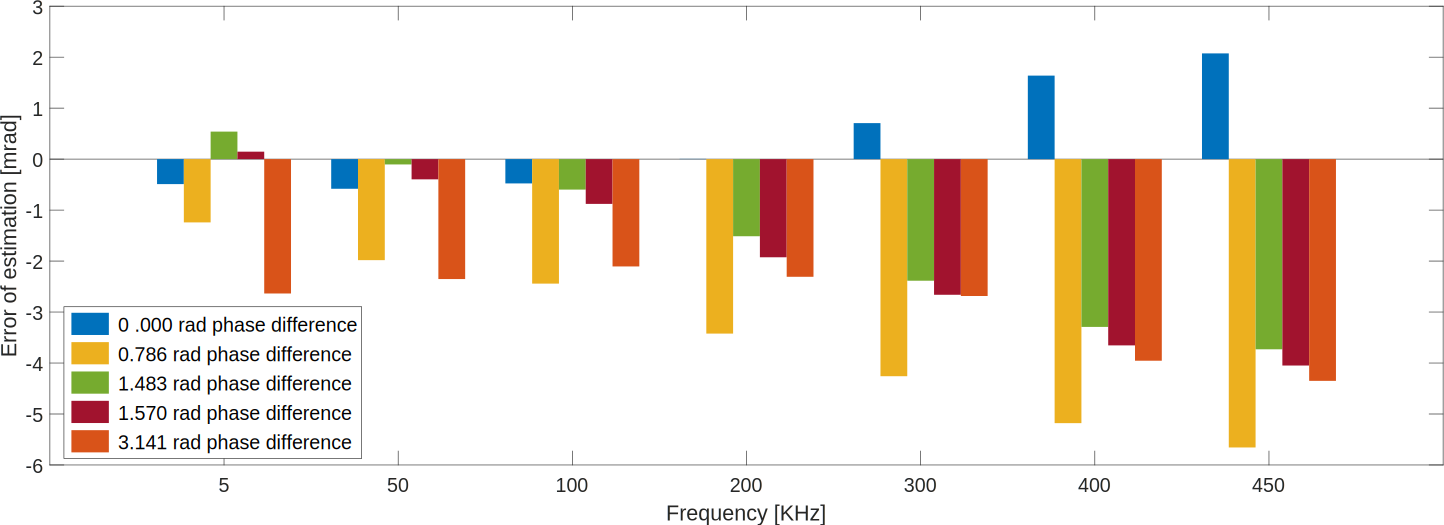
\includegraphics[width=1.1\linewidth]{phaseapproxerr.pdf}
\caption{Bar plot showing the error of estimation at \gls{if} frequencies of  5, 50, 100, 200, 300, 400, \SI{450}{\kilo\hertz} and different phase differences. The phase difference \SI{1.570}{\radian} should give an \gls{aoa} of 0 since this is a phase shift of \SI{90}{\degree}. The best precision is achieved at \SI{5}{\kilo\hertz} but \SI{50}{\kilo\hertz} still only introduces an error of \SI{0.40}{\milli\radian} at an \gls{aoa} of zero.}
\label{fig:app:aoaestimationerr}
\end{figure}